\documentclass[serif]{beamer}
\usetheme{Madrid}
\usepackage[utf8]{inputenc}
\usepackage{import, ragged2e, graphicx, enumerate, subfigure}
\usepackage{multicol, xcolor, amsmath, amsthm, array}
\usepackage{hyperref}

\newtheorem{mydef}{Definicão}
% Aling justify \item Itemize
\let\olditem\item
\renewcommand\item{\olditem\justifying}

% Título da Apresentação
\title{Cálculo IV}
\subtitle{Rotacional e Divergente}
\author{Leidivania / Mirely / Wellington}
\institute[]{Instituto Federal de Ciência e Tecnologia do Ceará - IFCE}
\date{Agosto - 2021}

% Índice da Apresentação
% \AtBeginSection[]
% {
%     \begin{frame}
%         \frametitle{Índice}
%         \tableofcontents[currentsection]
%     \end{frame}
% }

\begin{document}
\frame{\titlepage}
\begin{frame}
    \frametitle{Índice}
    \tableofcontents
\end{frame}

\section{Campo Vetorial em $R^3$}
\begin{frame}
    \frametitle{Campo Vetorial em $R^3$}
    \begin{mydef}
        Um campo vetorial no $\mathbb{R}^3$ é um aplicação $F: \Omega \rightarrow \mathbb{R}^3$, onde $\Omega \subset \mathbb{R}^3$.
    \end{mydef}
    \vspace{3mm}
    
    Nesse caso, o campo vetorial pode ser escrito em termos de suas componentes $P, Q, R$ da seguinte forma:
    
    \begin{equation*}
        F(x, y, z) = P(x, y, z) \vec{i} + Q(x, y, z) \vec{j} + R(x, y, z) \vec{k}
    \end{equation*}
    
    Onde, as funções reais de três variáveis $P, Q, R: \Omega$ são as funções componentes do campo vetorial.
    \vspace{3mm}
    
    É importante pensar em campo vetorial em $\mathbb{R}^3$ como uma função que associa, a cada ponto $x, y, z \in \Omega$ um vetor $F(x, y, z)$.
\end{frame}

\section{Rotacional}
\begin{frame}
    \frametitle{Rotacional}
    \begin{mydef}
        \justifying
        Considere um campo vetorial $\vec{F}: \Omega \rightarrow \mathbb{R}^3$, onde $\Omega \subset \mathbb{R}^3$, dado por $\vec{F}(x, y, z) = P(x, y, z)\vec{i} + Q(x, y, z)\vec{j} + R(x, y, z)\vec{k}$, onde $P, Q, R$ admitem derivadas parciais em $\Omega$. O rotacional de $\vec{F}$, indicado por $\nabla \times \vec{F}$ (ou $rot \vec{F}$) é o campo vetorial definido em $\Omega$ dado por:
    \end{mydef}
    
    \begin{equation*}
        \nabla \times \vec{F} = \left(
        \frac{\partial R}{\partial y} - \frac{\partial Q}{\partial z}
        \right)\vec{i} + \left(
        \frac{\partial P}{\partial z} - \frac{\partial R}{\partial x}
        \right)\vec{j} + \left(
        \frac{\partial Q}{\partial x} - \frac{\partial P}{\partial y}
        \right)\vec{k}
    \end{equation*}
    \vspace{3mm}
    
    Onde $\vec{i} = (1, 0, 0), \vec{j} = (0, 1, 0), \vec{k} = (0, 0, 1)$.
    
\end{frame}

\begin{frame}
    \frametitle{Rotacional}
    \justifying
    Na definição do slide anterior, utilizamos o operador $\nabla = \left(
        \dfrac{\partial}{\partial x},
        \dfrac{\partial}{\partial y},
        \dfrac{\partial}{\partial z}
        \right)$, chamado de operador \textit{Nabla}
    
    \begin{align*}
        \nabla \times \vec{F} & = \left|\begin{array}{ccc}
            \vec{i}                      & \vec{j}                      & \vec{k}                      \\[2mm]
            \dfrac{\partial}{\partial x} & \dfrac{\partial}{\partial y} & \dfrac{\partial}{\partial z} \\[4mm]
            P                            & Q                            & R
        \end{array}\right| \\[3mm]
                              & = \left(
        \dfrac{\partial R}{\partial y}-\dfrac{\partial Q}{\partial z}
        \right)\vec{i} + \left(
        \dfrac{\partial P}{\partial z}-\dfrac{\partial R}{\partial x}
        \right)\vec{j} + \left(
        \dfrac{\partial Q}{\partial x}-\dfrac{\partial P}{\partial y}
        \right)\vec{k}
    \end{align*}
    
\end{frame}

\begin{frame}
    \frametitle{Rotacional - Exemplos}
    \justifying
    \textbf{Exemplo 1:} Seja $\vec{F}(x, y, z)=2x^2y\vec{i}, 3xz\vec{j}, -y\vec{k}$. Neste caso, $P(x, y ,z)=2x^2y, Q(x, y, z)=3xz, R(x, y, z)=-y$. Então,
    
    \begin{align*}
        \nabla \times \vec{F} & = \left|\begin{array}{ccc}
            \vec{i}                      & \vec{j}                      & \vec{k}                      \\[2mm]
            \dfrac{\partial}{\partial x} & \dfrac{\partial}{\partial y} & \dfrac{\partial}{\partial y} \\[4mm]
            2x^2y                        & 3xz                          & -y
        \end{array}\right| \\[3mm]
                              & = \left(
        \dfrac{\partial (-y)}{\partial y}
        \vec{i} +
        \dfrac{\partial (2x^2y)}{\partial z}
        \vec{j} +
        \dfrac{\partial (3xz)}{\partial x}
        \vec{k}
        \right)
        \\[3mm]
                              & - \left(
        \dfrac{\partial(-y)}{\partial x}
        \vec{j} +
        \dfrac{\partial (3xz)}{\partial z}
        \vec{i} +
        \dfrac{\partial (2x^2y)}{\partial y}
        \vec{k}
        \right)
        \\[3mm]
                              & = (-1-3x)\vec{i} + (3z-2x^2)\vec{k}
    \end{align*}
\end{frame}

\begin{frame}
    \frametitle{Rotacional - Exemplos}
    \justifying
    \textbf{Exemplo 2:} Seja $\vec{F}(x,y,z)=(4x+5yz\vec{i}, 5xz\vec{j}, 5xy\vec{k})$. Nesse caso, $P(x,y,z)=4x+5yz, Q(x,y,z)=5xz, R(x,y,z)=5xy$. Então,
    
    \begin{align*}
        \nabla \times \vec{F} & = \left| \begin{array}{ccc}
            i                            & j                            & k                            \\[2mm]
            \dfrac{\partial}{\partial x} & \dfrac{\partial}{\partial y} & \dfrac{\partial}{\partial z} \\[4mm]
            4x+5yz                       & 5xz                          & 5xy
        \end{array}\right|                \\[3mm]
                              & = \left(
        \dfrac{\partial (5xy)}{\partial y}
        \vec{i} +
        \dfrac{\partial (4x+5yz)}{\partial z}
        \vec{j} +
        \dfrac{\partial (5xz)}{\partial x}
        \vec{k}
        \right)
        \\[3mm]
                              & - \left(
        \dfrac{\partial (5xy)}{\partial x}
        \vec{j} +
        \dfrac{\partial (5xz)}{\partial z}
        \vec{i} +
        \dfrac{\partial (4x+5yz)}{\partial y}
        \vec{k}
        \right)
        \\[3mm]
                              & = (5x-5x)\vec{i}+(5y-5y)\vec{j}+(5z-5z)\vec{k} = \vec{0}
    \end{align*}
\end{frame}

\section{Divergente}
\begin{frame}
    \frametitle{Divergente}
    \begin{mydef}
        \justifying
        Seja $\vec{F}=(P,Q,R)$ um campo vetorial definido em $\Omega \subset \mathbb{R}^3$. Suponha que $P,Q,R$ admitem derivadas parciais em $\Omega$. O divergente de $\vec{F}$, indicado por $\nabla \cdot \vec{F}$ (ou $div \vec{F}$) é o campo vetorial dado por:
        \begin{equation*}
            \nabla \cdot \vec{F} = \dfrac{\partial P}{\partial x}+\dfrac{\partial Q}{\partial y}+\dfrac{\partial R}{\partial z}
        \end{equation*}
    \end{mydef}
    
    A expressão acima é dada por:
    
    \begin{align*}
        \nabla \cdot \vec{F} & = \left(\dfrac{\partial}{\partial x},\dfrac{\partial}{\partial y},\dfrac{\partial}{\partial z}\right) \cdot (P,Q,R) \\[3mm]
                             & = \dfrac{\partial P}{\partial x}+\dfrac{\partial Q}{\partial y}+\dfrac{\partial R}{\partial z}
    \end{align*}
    
\end{frame}

\begin{frame}
    \frametitle{Divergente}
    
    A definição do slide anterior pode ser generalizada. 
    \vspace{5mm}
    
    Se $\vec{F}=(F_1, F_2, \ldots, F_n)$, então definimos o divergente de $\vec{F}$ por
    \vspace{3mm}
    
    \begin{equation*}
        \nabla \cdot \vec{F} = \sum\limits_{i=1}^{n} \dfrac{\partial Fi}{\partial xi}.
    \end{equation*}
\end{frame}

\section{Divergente - Exemplos}
\begin{frame}
    \frametitle{Divergente - Exemplos}
    \justifying
    \textbf{Exemplo 1:} Seja $\vec{F}(x,y,z)=(x^2y\vec{i}, 2xy\vec{j}, z^2\vec{k})$. Neste caso, $P(x,y,z)=x^2y, Q(x,y,z)=2xy, R(x,y,z)=z^2$
    
    \begin{align*}
        \nabla \cdot \vec{F} & =\left(
        \dfrac{\partial}{\partial x}, \dfrac{\partial}{\partial y}, \dfrac{\partial}{\partial z}
        \right) \cdot (x^2y,2xy,z^2)                                                                                                 \\[3mm]
                             & = \dfrac{\partial x^2y}{\partial x}+\dfrac{\partial 2xy}{\partial y}+\dfrac{\partial z^2}{\partial z} \\[3mm]
                             & = 2xy+2x+2z
    \end{align*}
    
\end{frame}

\begin{frame}
    \frametitle{Divergente - Exemplos}
    \justifying
    \textbf{Exemplo 2:} Seja $\vec{F}(x,y,z)=\dfrac{-mMG}{r^3}(x,y,z)$, onde $m, M, G$ são constantes positivas. 
    
    Nesse caso, $P(x,y,z)=\dfrac{-mMGx}{r^3}, Q(x,y,z)=\dfrac{-mMGy}{r^3}, R(x,y,z)=\dfrac{-mMGz}{r^3}$
    
    \begin{align*}
        \nabla \cdot \vec{F} & = \left(
        \dfrac{\partial}{\partial x}, \dfrac{\partial}{\partial y}, \dfrac{\partial}{\partial z}
        \right) \cdot \left(
        \dfrac{-mMGx}{r^3}, \dfrac{-mMGy}{r^3}, \dfrac{-mMGz}{r^3}
        \right)                                                                                                                                                                  \\[2mm]
                             & = \dfrac{\partial \dfrac{-mMGx}{r^3}}{\partial x}+\dfrac{\partial \dfrac{-mMGy}{r^3}}{\partial y}+\dfrac{\partial \dfrac{-mMGz}{r^3}}{\partial z} \\[2mm]
                             & = \dfrac{-mMGr^3}{r^6}+\dfrac{-mMGr^3}{r^6}+\dfrac{-mMGr^3}{r^6}                                                                                  \\[2mm]
                             & = \dfrac{-3mMGr^3}{r^6} = \dfrac{-3mMG}{r^3}
    \end{align*}
\end{frame}
\section{A história do Teorema da divergência}
\begin{frame}
    \frametitle{A história do teorema da divergência}
    \begin{itemize}
        \item \textbf{George Green (1793-1841)}:
              \begin{itemize}
                  \item Matemático autodidata
                  \item "Um ensaio sobre a aplicação da análise matemática às Teorias de Elasticidade e Magnetismo."
              \end{itemize}
        \item \textbf{Gauss (1777-1855)}:
              \begin{itemize}
                  \item Príncipe dos matemáticos
                  \item Teorema de Gauss
              \end{itemize}
        \item \textbf{Michal V. Ostrogradskij (1801-1861)}:
              \begin{itemize}
                  \item Declarou e provou a fórmula
              \end{itemize}
    \end{itemize}
\end{frame}

\begin{frame}
    \frametitle{A história do teorema de Stokes}
    \begin{itemize}
        \item \textbf{Stokes (1819-1903):}
              \begin{itemize}
                  \item Referência em dinâmica dos fluídos, óptica e física matemática
                  \item Utiliza o rotacional em seu teorema e fórmula
              \end{itemize}
    \end{itemize}
    \vspace{5mm}
    \begin{equation*}
        \oint_C F \cdot dr = \iint_S rot F dS
    \end{equation*}
\end{frame}

\section{Aplicações}
\begin{frame}
    \frametitle{Aplicações}
    \begin{itemize}
        \item Mecânica dos fluídos
        \item Eletricidade
        \item Magnetismo
    \end{itemize}
\end{frame}

\section{Interpretação física do rotacional}
\begin{frame}
    \frametitle{Interpretação física do rotacional}
    \begin{itemize}
        \item A razão para o nome \textit{rotacional} é que o vetor rotacional está associado com rotações.
        \item Outra ocorre quando $F$ representa um campo de velocidade em mecânica dos fluidos.
        \item O rotacional de um campo de vetores que representa a velocidade de um fluido, está relacionado ao fenômeno de rotação do fluído. Existe uma relação entre rotacional e aspectos rotacionais do movimento.
    \end{itemize}
\end{frame}

\begin{frame}
    \frametitle{Interpretação física do rotacional}
    Seja $F$ um campo de vetores que representa o campo de velocidade de um fluido e consideramos uma partícula situada no ponto $\vec{F}$.
    \vspace{3mm}
    
    As particulas situadas num vizinhança deste ponto, tendem a rodar em torno do eixo que aponta na direção do $\text{\textit{rot}} \vec{F}(x,y,z)$, e o comprimento desse vetor rotacional é a medida de quão rápido as partículas se movem em torno desse eixo.
    
    \begin{figure}[h]
        \centering
        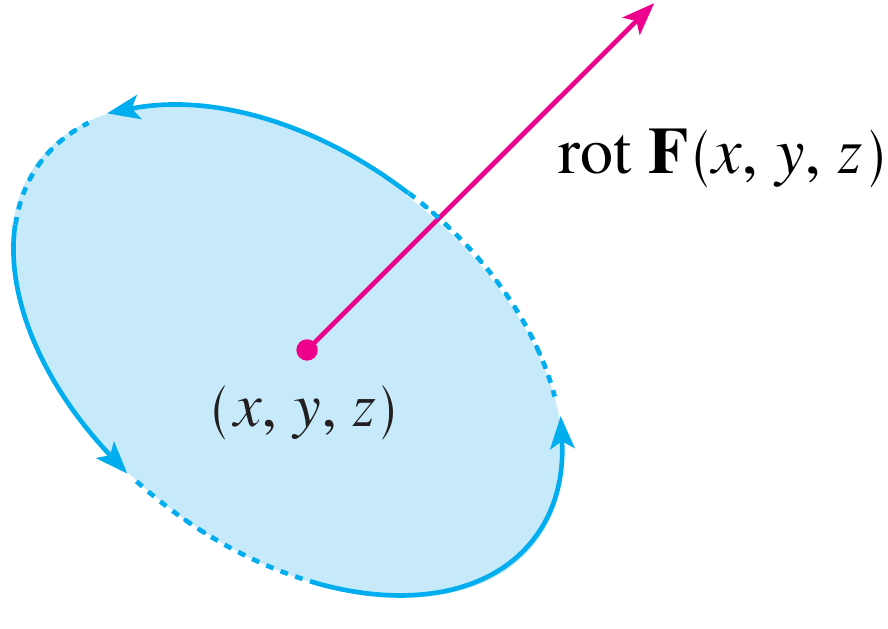
\includegraphics[scale=0.2]{img/rotacional.png}
    \end{figure}
\end{frame}

\begin{frame}
    \frametitle{Interpretação física do rotacional}
    \justifying
    Como já dito, o rotacional pode ter sua representação física relacionada à capacidade de giro que uma parte infinitesimal de um campo vetorial apresenta. Para auxiliar na visualização, vamos imaginar um campo vetorial qualquer, tomo como exemplo a função $F(x,y)=-y\vec{i}+x\vec{j}$.
    
    \begin{figure}[h]
        \centering
        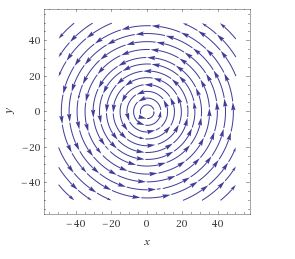
\includegraphics[scale=0.7]{img/Campo_Vetorial.jpg}
    \end{figure}
\end{frame}

\begin{frame}
    \frametitle{Interpretação física do rotacional}
    \justifying
    Então é colocado um disco dentro da água, e este disco tem um \textit{"Norte"}, que consiste no seu sentido de orientação. Ao ser colocado dentro do campo vetorial o disco começa a se movimentar de forma circular, acompanhando o deslocamento da água, mas sem mudar seu sentido e direção, mantendo seu \textit{"Norte"}. Este campo é dado como irrotacional.
    
    \begin{figure}[h]
        \centering
        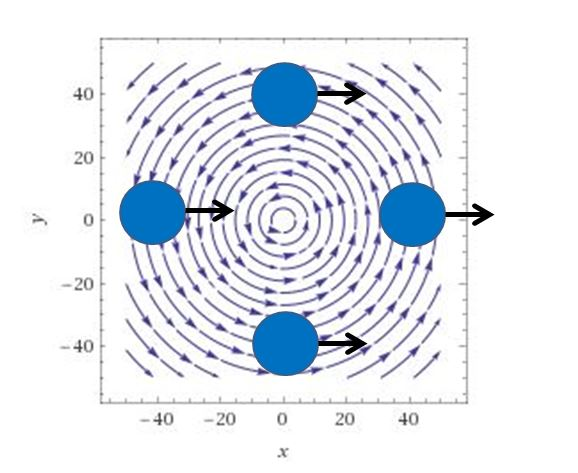
\includegraphics[scale=0.4]{img/Campo_Vetorial_com_Disco.jpg}
    \end{figure}
\end{frame}

\begin{frame}
    \frametitle{Interpretação física do rotacional}
    \justifying
    Agora imagine que outro disco é colocado dentro da água, só que desta vez, o centro do disco começa a se movimentar e girar em torno do seu prórpio eixo, ao longo do seu movimento, seu \textit{"Norte"} muda de sentido e direção. Esta capacidade do disco girar ao longo do movimento pode ser interpretada como o rotacional do campo vetorial.
    
    \begin{figure}[h]
        \centering
        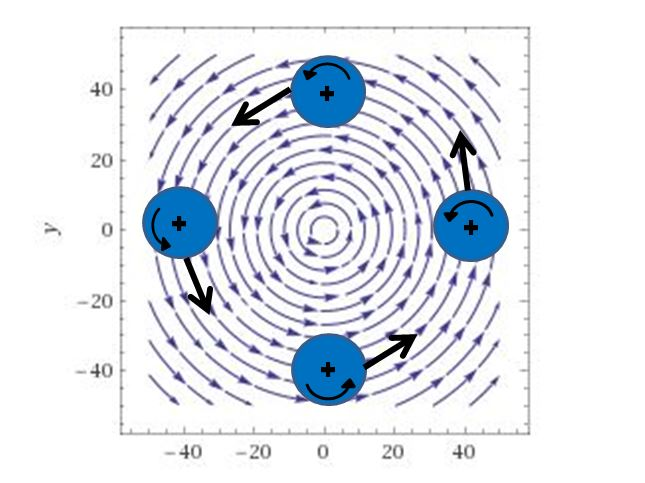
\includegraphics[scale=0.4]{img/Campo_Vetorial_com_Disco_Girando.jpg}
    \end{figure}
\end{frame}

\begin{frame}
    \frametitle{Interpretação física do rotacional}
    \justifying
    O rotacional pode ser obtido através da regra da mão direita, em que se posicionam os 4 dedos acompanhando o movimento de giro do disco, e por consequência, o polegar acaba apontando na direção do rotacional. No caso do disco, utilizando a regra, conclui-se que o rotacional está apontando para o eixo $\vec{k}$ positivo, isto é, para fora.
    
    \begin{figure}[h]
        \centering
        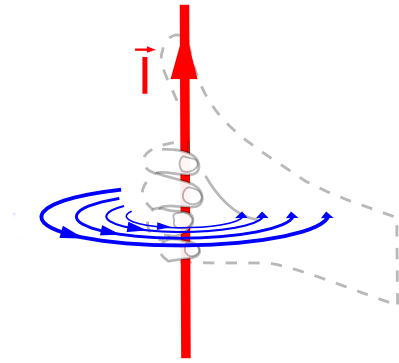
\includegraphics[scale=0.3]{img/Right_hand_rule.png}
    \end{figure}
\end{frame}

\begin{frame}
    \frametitle{Interpretação física do rotacional}
    \justifying
    Para o campo $F(x,y)$ dado, tem-se:
    
    \begin{displaymath}
        \nabla \times \vec{F} = \left| \begin{array}{ccc}
            \vec{i}                     & \vec{j}                     & \vec{k}                     \\[3mm]
            \frac{\partial}{\partial x} & \frac{\partial}{\partial y} & \frac{\partial}{\partial z} \\[3mm]
            -y                          & x                           & 0
        \end{array}\right|
    \end{displaymath}
    Calculando-se então o determinante:
    \begin{equation*}
        det = \left(
        \frac{\partial}{\partial y} \cdot 0 - \frac{\partial}{\partial z} \cdot x
        \right)\vec{i} + \left(
        \frac{\partial}{\partial z} \cdot (-y) - \frac{\partial}{\partial x} \cdot 0
        \right)\vec{j} + \left(
        \frac{\partial}{\partial x} \cdot x - \frac{\partial}{\partial x} \cdot (-y)
        \right)\vec{k}
    \end{equation*}
    Calculando as derivadas, tem-se então:
    \\[3mm]
    $det = (0-0)\vec{i}+(0-0)\vec{j}+(1+1)\vec{k}$
\end{frame}
\section{Interpretação física do divergente}
\begin{frame}
    \frametitle{Interpretação física do divergente}
    A divergência mede a mudança na densidade de um liquido escoando de acordo com um dado campo vetorial.
    
    \begin{itemize}
        \item Interprete um campo vetorial como representando o escoamento de um fluido.
        \item A divergência é um operador que tem como entrada a função vetorial que define esse campo e dá como saída um função escalar que mede a variação da densidade do fluido em cada ponto do campo.
        \item Fórmulo da divergência:
              \begin{equation*}
                  div \vec{F} = \nabla \cdot \vec{F} = \dfrac{\partial F_1}{\partial x}+\dfrac{\partial F_2}{\partial y}+ \cdots
              \end{equation*}
        \item Onde, $F_1, F_2, \ldots$ são funções componentes de $\vec{F}$.
    \end{itemize}
\end{frame}

\begin{frame}
    \frametitle{Interpretação física do divergente}
    Digamos que, ao calcular a divergência de um função $\vec{F}$ em um certo ponto $(x_0,y_0)$, encontramos um valor negativo.
    \vspace{2mm}
    
    \begin{equation*}
        \nabla \cdot \vec{F}(x_0,y_0) < 0
    \end{equation*}
    \vspace{2mm}
    
    Isso significa que um fluido escoando segundo o campo vetorial definido por $\vec{F}$ tenderia a ficar \textbf{mais denso} no ponto $(x_0,y_0)$.
    \vspace{5mm}
    
    \textbf{Animação de um campo com divergência negativa na origem:}
    \begin{itemize}
        \item \href{https://www.youtube.com/watch?v=rqnTQyO4GY4}{Divergente Negativo}
    \end{itemize}
    
\end{frame}

\begin{frame}
    \frametitle{Interpretação física do divergente}
    Por outro lado, se a divergência no ponto $(x_0,y_0)$ for positiva,
    \vspace{2mm}
    
    \begin{equation*}
        \nabla \cdot \vec{F}(x_0,y_0) > 0
    \end{equation*}
    \vspace{2mm}
    
    o fluido escoando de acordo com o campo vetorial se torna menos denso ao redor de $(x_0,y_0)$.
    \vspace{5mm}
    
    \textbf{Animação de um campo com divergência positiva:}
    \begin{itemize}
        \item \href{https://www.youtube.com/watch?v=_mwMoEwwkvc}{Divergente Positivo}
    \end{itemize}
    
\end{frame}

\begin{frame}
    \frametitle{Interpretação física do divergente}
    Por fim, o conceito de divergência nula, ele indica que até mesmo se um fluido estiver escoando livremente, sua densidade se mantêm constante. Conveniente quando se modela fluido incompressível, como a água.
    \vspace{2mm}
    
    \begin{equation*}
        \nabla \cdot \vec{F} = 0
    \end{equation*}
    \vspace{2mm}
    
    Tais campos vetoriais são chamados de "divergência nula".
    \vspace{5mm}
    
    \textbf{Animação de como o campo deve se parecer:}
    \begin{itemize}
        \item \href{https://www.youtube.com/watch?v=TC9MP-y1s_c}{Fluido incompressível}
    \end{itemize}
    
\end{frame}

\begin{frame}
    \frametitle{Fontes e Sumidouros}
    \justifying
    Da mesma forma, ao invés de pensar nos pontos com divergência positiva como se tornando menos densos durante um movimento momentâneo, esses pontos podem ser vistos como "fontes", constantemente gerando mais partículas do fluido.
    \vspace{3mm}
    
    \begin{equation*}
        \nabla \cdot \vec{F}(x_0,y_0) < 0
    \end{equation*}
    \vspace{3mm}
    
    \textbf{Animação de como deve ser a aparência de sumidouros}
    \begin{itemize}
        \item \href{https://www.youtube.com/watch?v=4I5R4zhOzmU}{Sumidouros}
    \end{itemize}
    
\end{frame}

\begin{frame}
    \frametitle{Fontes e Sumidoros}
    \justifying
    Às vezes, nos pontos com divergência negativa, ao invés de pensar em um fluido ficando mais denso após um movimento momentâneo, algumas pessoas imaginam o fluido sendo drenado naquele ponto enquanto o fluido escoa constantemente.
    \vspace{3mm}
    
    \begin{equation*}
        \nabla \cdot \vec{F}(x_0,y_0) > 0
    \end{equation*}
    \vspace{3mm}
    
    \textbf{Animação de como deve ser a aparência de fontes}
    \begin{itemize}
        \item \href{https://www.youtube.com/watch?v=mBoezvLrUGw}{Fontes}
    \end{itemize}
    
\end{frame}
\section{Time}
\begin{frame}
    \frametitle{Time}
    \begin{itemize}
        \item Leidivania
        \item Mirely
        \item Wellington
    \end{itemize}
\end{frame}

\end{document}